\section{Theoretical Analysis}

In this analysis, we have some differences from the theoretical analysis for some of the standard parts of an AC-DC converter, those being the high number of diodes and the absence of the resistor in parallel with the capacitor.

Initially we started with a voltage source with the standard $\frac{230}{n}V$ and $50Hz$, in which $n$ was the one experimentally determined to produce the best merit in ngspice, in this case being $17.78988$, which produces an amplitude of $12.9287$.

The first part of the circuit to be analysed is the full-wave rectifier, which has a behaviour that is well described by the absolute value of the input wave, because the voltage is way bigger than $V_{ON}$ of the diode.

\begin{equation}
    V_{Full Wave} = \left|\frac{V_in}{n}\right|
    \label{eq:fullwave_mat}
\end{equation}

The next component is the capacitor has a envelope detector. The formula for calculating the envelope voltage in each period is 

\begin{equation}
    V_{envelope}=A\cos{(\omega t_{OFF})}e^{-\frac{t_{ON}-t_{OFF}}{RC}}
\end{equation}

with 

\begin{equation}
    t_{OFF}=\frac{1}{\omega}\arctan\left(\frac{1}{\omega R C}\right)
\end{equation}

But in our circuit we did not included the resistor so, with it being in parallel it will behave not as if the resistance is infinite but as the resistance that still exist in the diodes that is very high because we chose to use then even bellow $V_{ON}$. This being said, the resistance used in this formula for this specific analysis is $N r_d$, with $r_d$ as determined in the next section, equation \eqref{eq:rad_mat}.

\begin{figure}[H]
    \centering
    \includegraphics[width = 0.85\linewidth]{mat/antes_mat.png}
        \caption{\textit{Signal as it exits the envelope detector according to the theoretical analysis.}}
    \label{fig:plot6}
\end{figure}

The last part of the circuit is the voltage regulator, in our case it's a set of 31 diodes in series, all in parallel with the capacitor. In this analysis we followed the expected formulae, although, because of the heavy difference between simulation and theoretical analysis we can begin disprove the usage of these equations for higher number of diodes.

First we must understand the behavior of the diodes and the best way to understand it it through it's incremental resistance, it starts of as really high but than it decreases to more constant and low values and this change is exponential. That being said, the formula is the following. 

\begin{equation}
    r_d = \frac{\eta V_T}{I_S e^{\frac{V_D}{\eta V_T}}}
    \label{eq:rad_mat}
\end{equation}

\begin{figure}[H]
\hspace{-10mm}
  \subfigure[Current as function of voltage]{% 
    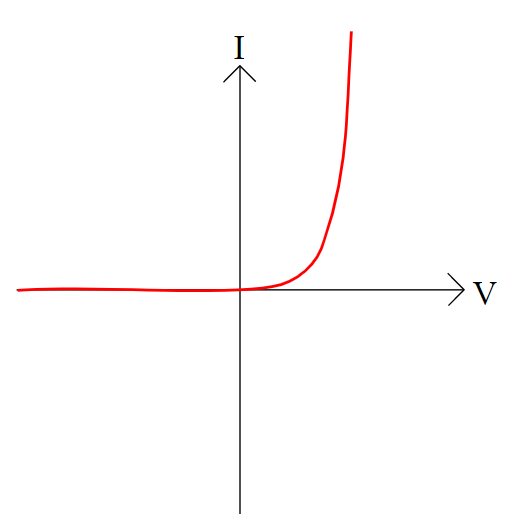
\includegraphics[width=.45\textwidth]{diode.png} \label{fig:diode} 
  } 
  \subfigure[Voltage as function of current]{% 
    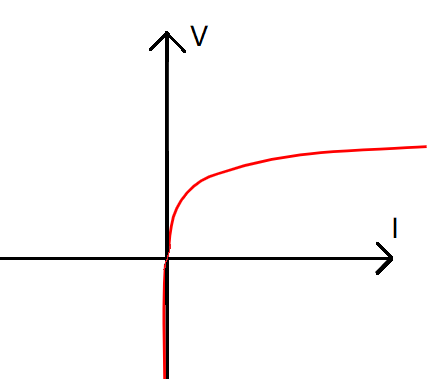
\includegraphics[width=.5\textwidth]{diode_R.png} \label{fig:diode_R} 
  } 
  \caption{I-V characteristic of a diode} 
\end{figure}

In this figure we can both understand that the diodes have different regions depending on the voltage but, considering $R=\frac{dV}{dI}$, from the second figure we conclude that the resistance if extremely high for the OFF zone of the diode and it can be used as a high resistance instead of actual resistors.

with $\eta=1$, $V_T = 0.025V$, $I_S=10^-{14}$ and $V_D$ being the the voltage difference in each diode that the estimated as being the value in the input of the set of diodes divided by the number of diodes. And, as expected we obtained a big value that is 247280.745039$\Omega$. The biggest difference to the simulation analysis starts here: the high number of diodes seems to help stabilize the signal, but the following formula indicates that for high number of diodes and diode incremental resistance the oscillation after the voltage regulator must be the same as the one leaving the envelope detector

\begin{equation}
    v_o = \frac{N r_d}{N r_d + R}V_{envelope}
    \label{eq:v_o_mat}
\end{equation}

The only thing left to discuss is the DC component of this approximation for the voltage regulator which will be $V_{envelope}$ unless $V_{envelope}$ is bigger than $N V_{ON}$, but $V_{ON}$ is some value between $0.65$ and $0.7$ $k\Omega$ so it's upper limit with $N=31$ is way higher than any value in $V_{envelope}$, so the DC component is only change, and just a little, in the oscillation amplitude from the previous formula.


\begin{figure}[H]
    \centering
    \includegraphics[width = 0.85\linewidth]{mat/zauzau_mat.png}
        \caption{\textit{Output voltage according to the theoretical analysis.}}
    \label{fig:plot3}
\end{figure}

\begin{figure}[H]
    \centering
    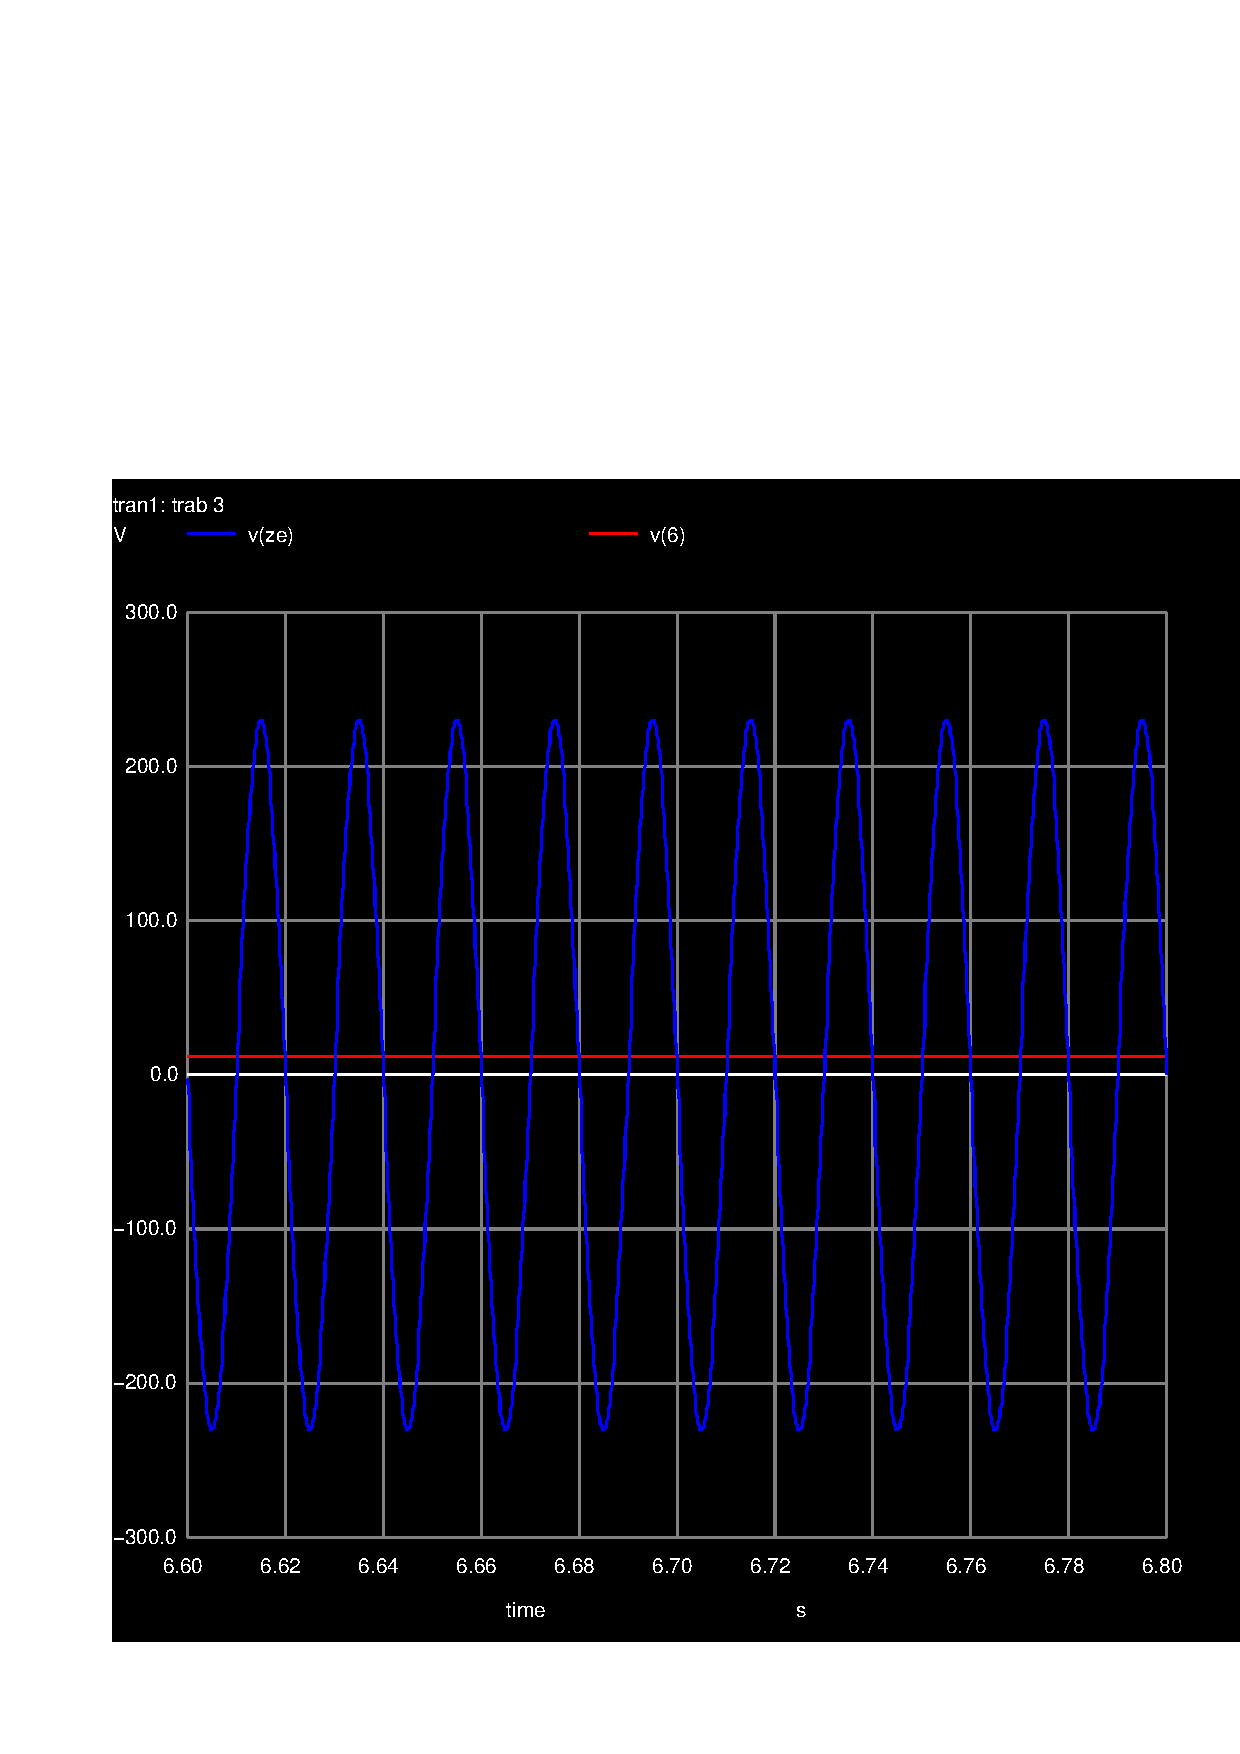
\includegraphics[width = 0.85\linewidth]{mat/acdc.png}
        \caption{\textit{Comparison between output and input voltage.}}
    \label{fig:plot4}
\end{figure}

\begin{figure}[H]
    \centering
    \includegraphics[width = 0.85\linewidth]{mat/deviation_mat.png}
        \caption{\textit{Output signal minus the 12V goal.}}
    \label{fig:plot5}
\end{figure}

With this output and the components used the final relevant values are the average of the signal 12.922513V, the ripple 0.025281V and finally the merit 0.232528, but as we know the value of the average can be easily adjusted by n in the transformer so, removing that term, the corrected merit in the theoretical analysis is 8.542956.